\chapter{Sources of Systematic Uncertainty}\label{ch:systematics}

Sources of systematic uncertainty associated with the real background prediction, fake background measurement, and signal calculation are considered. These uncertainties either affect the shape or normalization of the corresponding distribution and are applied to the final selection.

\section{Real Background Systematic Uncertainties}

The SM diphoton background prediction is performed at NNLO accuracy, but higher order terms could still contribute. To account for this, we allow the normalization of this predicted background to float freely, constrained only by the data. The fit is primarily constrained at low \mgg, where the statistical uncertainty on the data is the smallest. Potential signals are expected in the high-\mgg region and, provided the signal and background shapes differ significantly, this technique will discriminate between the two, as is the case in this analysis. In addition, allowing the background normalization to float will absorb the systematic uncertainties associated with the integrated luminosity measurement and inefficiencies from the trigger and high-\pt photon ID selection. These uncertainties are small and must be applied to the signal calculation, since its normalization is not allowed to float freely, as described below. The details regarding how the fit is performed will be presented in Chapter~\ref{ch:results}.

Systematic uncertainties on the shape of the SM background prediction are determined by varying the scales used in the \Kfactor calculation, separately for the EBEB and EBEE regions. As described in Section~\ref{sec:k_factor}, the renormalization, factorization, and fragmentation scales are varied simultaneously between $\mgg/2$ and $2\mgg$, from their default value of \mgg. Within the \MCFM framework, these scales affect the differential cross section via an estimate of the truncation of the perturbative calculation, the transition point between the hard calculation and the PDFs, and the fragmentation functions, respectively. Fig.~\ref{fig:kfactor_comparison_NNLO} shows each \Kfactor corresponding to the different choice of scales. The uncertainty increases with \mgg and, in general, is larger in the EBEE region.

\begin{figure}[hbtp!]
  \centering
  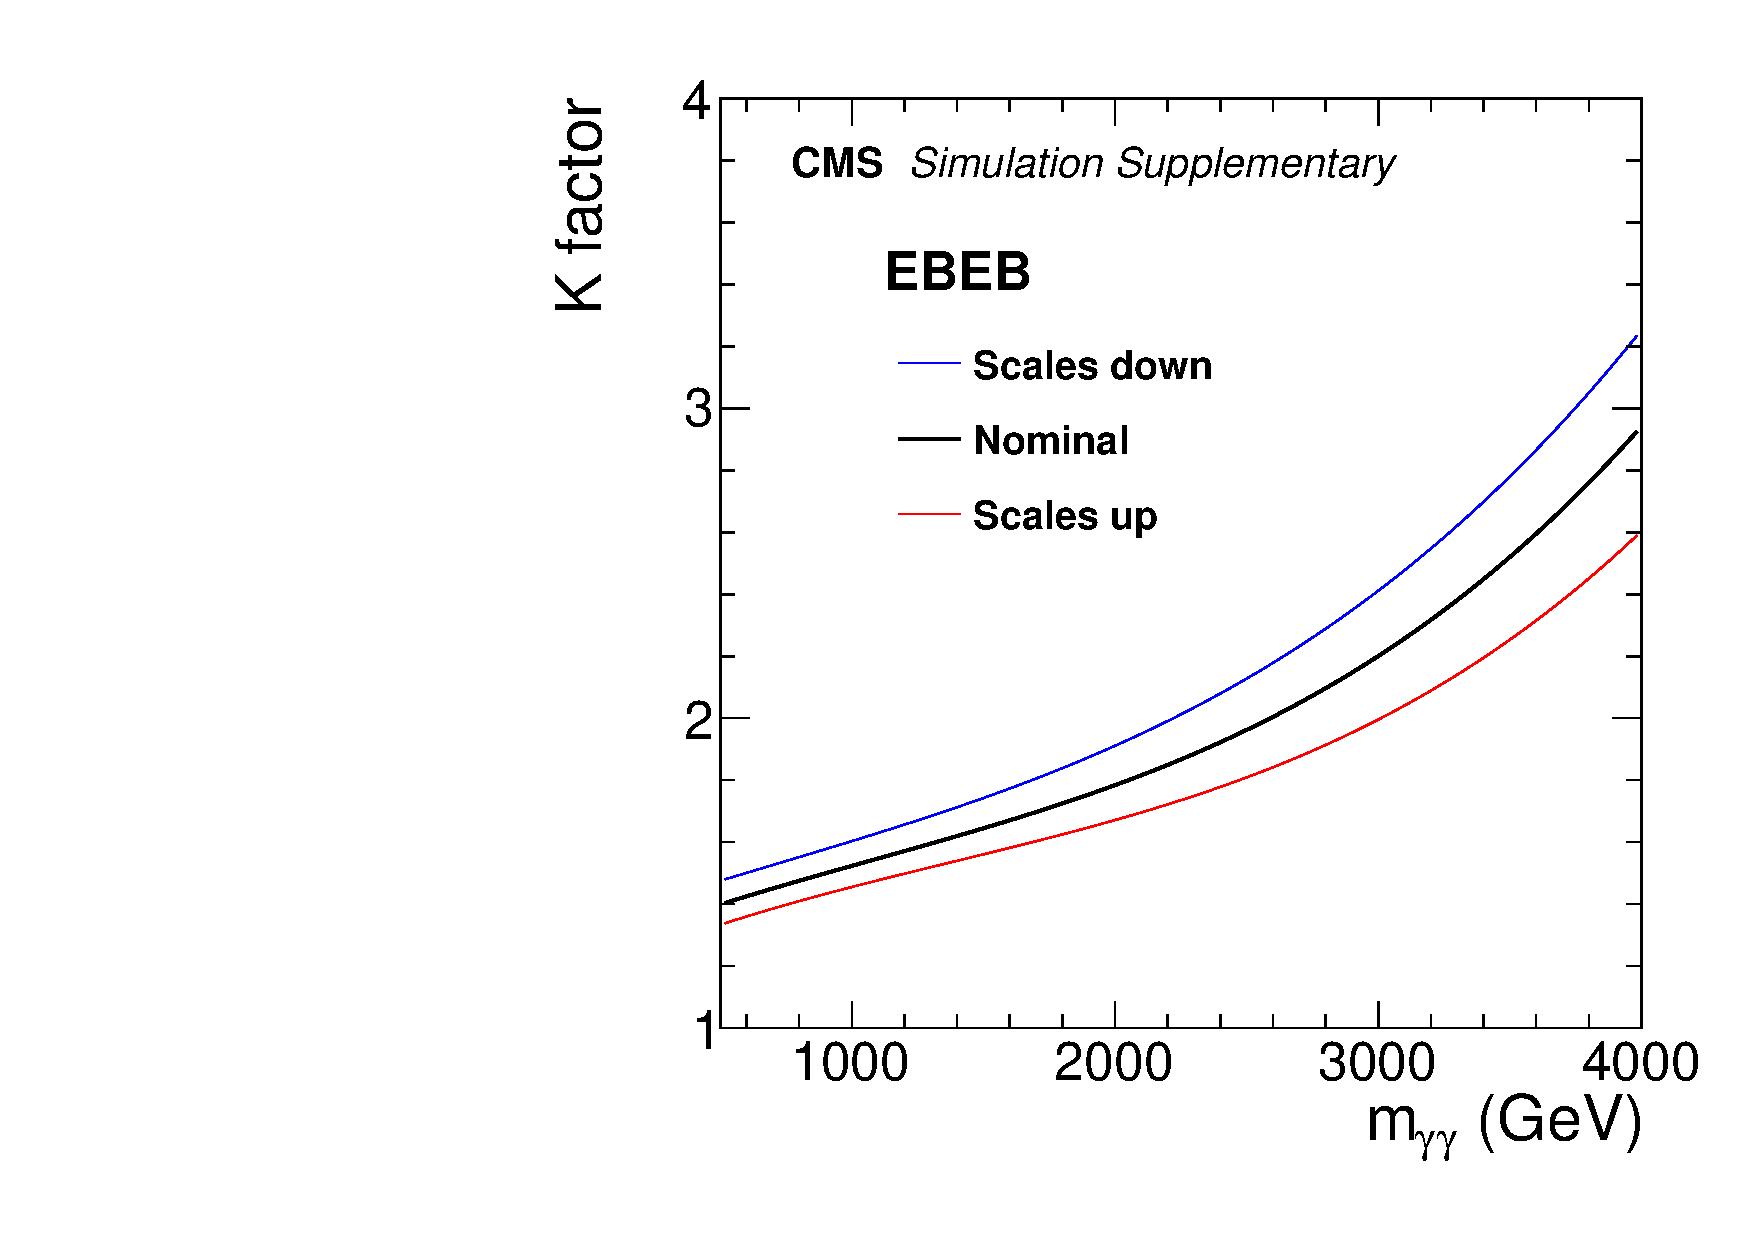
\includegraphics[width=0.49\textwidth]{figures/kfactorScaleVariations_BB.pdf}
  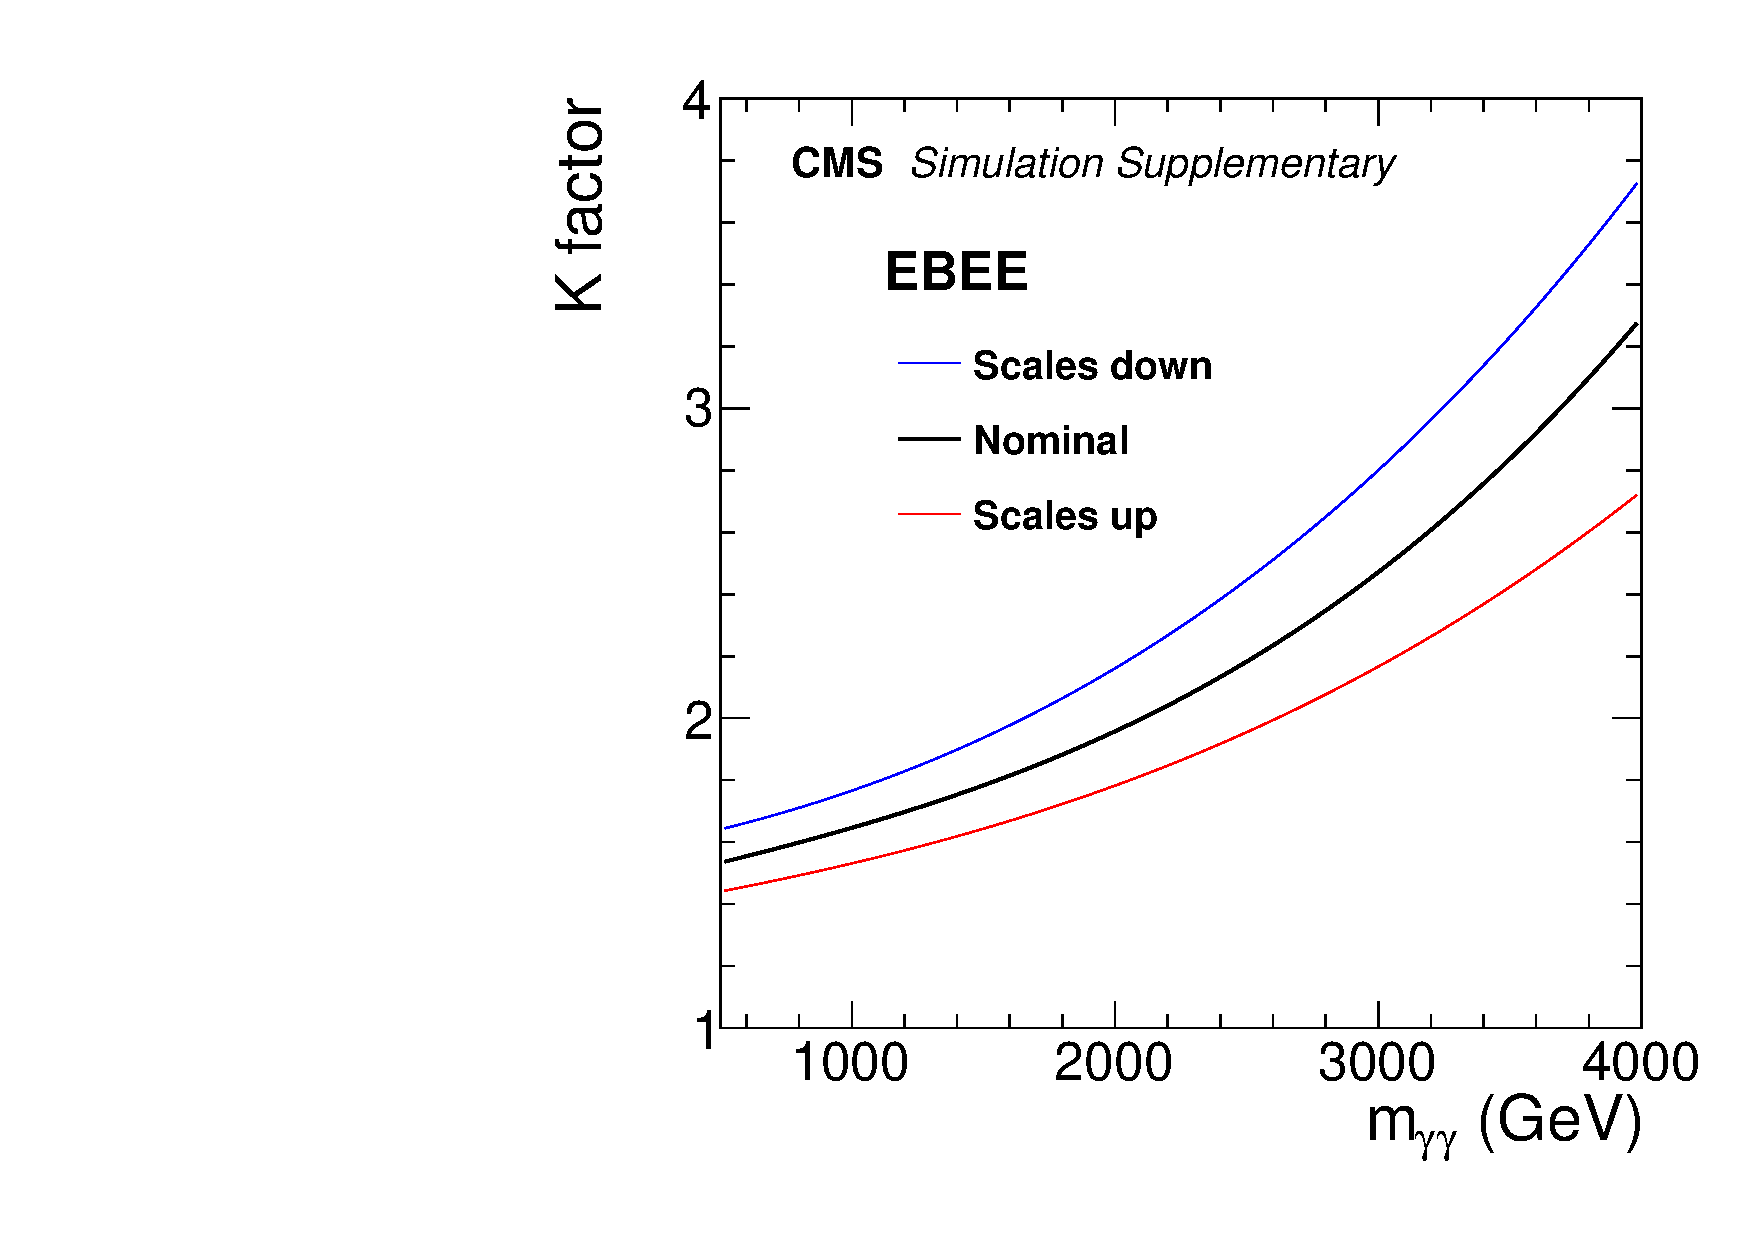
\includegraphics[width=0.49\textwidth]{figures/kfactorScaleVariations_BE.pdf}
  \caption{The \Kfactor as a function of \mgg in the EBEB (left) and EBEE (right) categories. The \Kfactor is defined as the ratio of the predicted \MCFM NNLO $\mathrm{pp} \to \gamma\gamma$ cross section to that of \SHERPA. The renormalization and factorization scales have been set to \mgg (black) and varied simultaneously by factors of 0.5 (blue) and 2.0 (red).}
  \label{fig:kfactor_comparison_NNLO}
\end{figure}

Systematic uncertainties on the SM background shape associated with the PDFs are calculated using the fixed-order, parton-level MC program \DIPHOX~\cite{Binoth:1999qq}, at NLO with a consistent set of CT10 NLO PDFs as used by \MCFM. \DIPHOX uses fragmentation functions with a cone-based photon isolation, meaning that the isolation energy within the cone is less than a constant value (5\GeV), yielding results consistent with the Frixione isolation configured in \MCFM. \DIPHOX only calculates up to NLO and is used primarily for computational convenience. Checks were performed to ensure that \DIPHOX at NLO agreed with \MCFM at NLO. The CT10 NLO set of PDFs contains 26 eigenvector pairs, each of which are individually varied by $\pm1$ standard deviation around its nominal value. Each eigenvector is treated as a separate systematic uncertainty, yielding 52 individual systematic uncertainties, all fully correlated as a function of \mgg. For each eigenvector variation, the ratio of the \mgg distribution obtained with that variation using \DIPHOX at NLO to that of the default distribution using \MCFM at NNLO is used to reweight the \MCFM SM diphoton background prediction, yielding a shape uncertainty. The variations for each eigenvector pair are shown in Figs.~\ref{fig:sys_PDF_EB} and~\ref{fig:sys_PDF_EE} for the EBEB and EBEE categories, respectively. In general the variations increase and can become large at high-\mgg (above 3\TeV). This is expected since experimental data is used as an input to improve PDF calculations, and the LHC is currently probing the highest energy scales, so is yet to provided any data in these very high regions. As a simplified check of this method, the NNLO cross section was calculated using \MCFM following the PDF4LHC prescription with the PDF4LHC15\_mc set of PDFs~\cite{Butterworth:2015oua}. This technique uses the PDF4LHC master formulas~\cite{Butterworth:2015oua}, which combine the separate uncertainties. The difference between the NNLO cross sections calculated assuming the CT10 and PDF4LHC15\_mc sets of PDFs were found to be within the assigned uncertainty from this method.

\begin{figure}[!htbp]
	\centering
	\includegraphics[scale=0.20]{figures/SYS_PDF_EB.pdf}
	\caption{The $\pm1$ standard deviation variations of each of the 26 PDF eigenvectors in the EBEB category. Each distribution is the ratio of the variation over the default prediction as a function of \mgg.}
	\label{fig:sys_PDF_EB}
\end{figure}

\begin{figure}[!htbp]
	\centering
	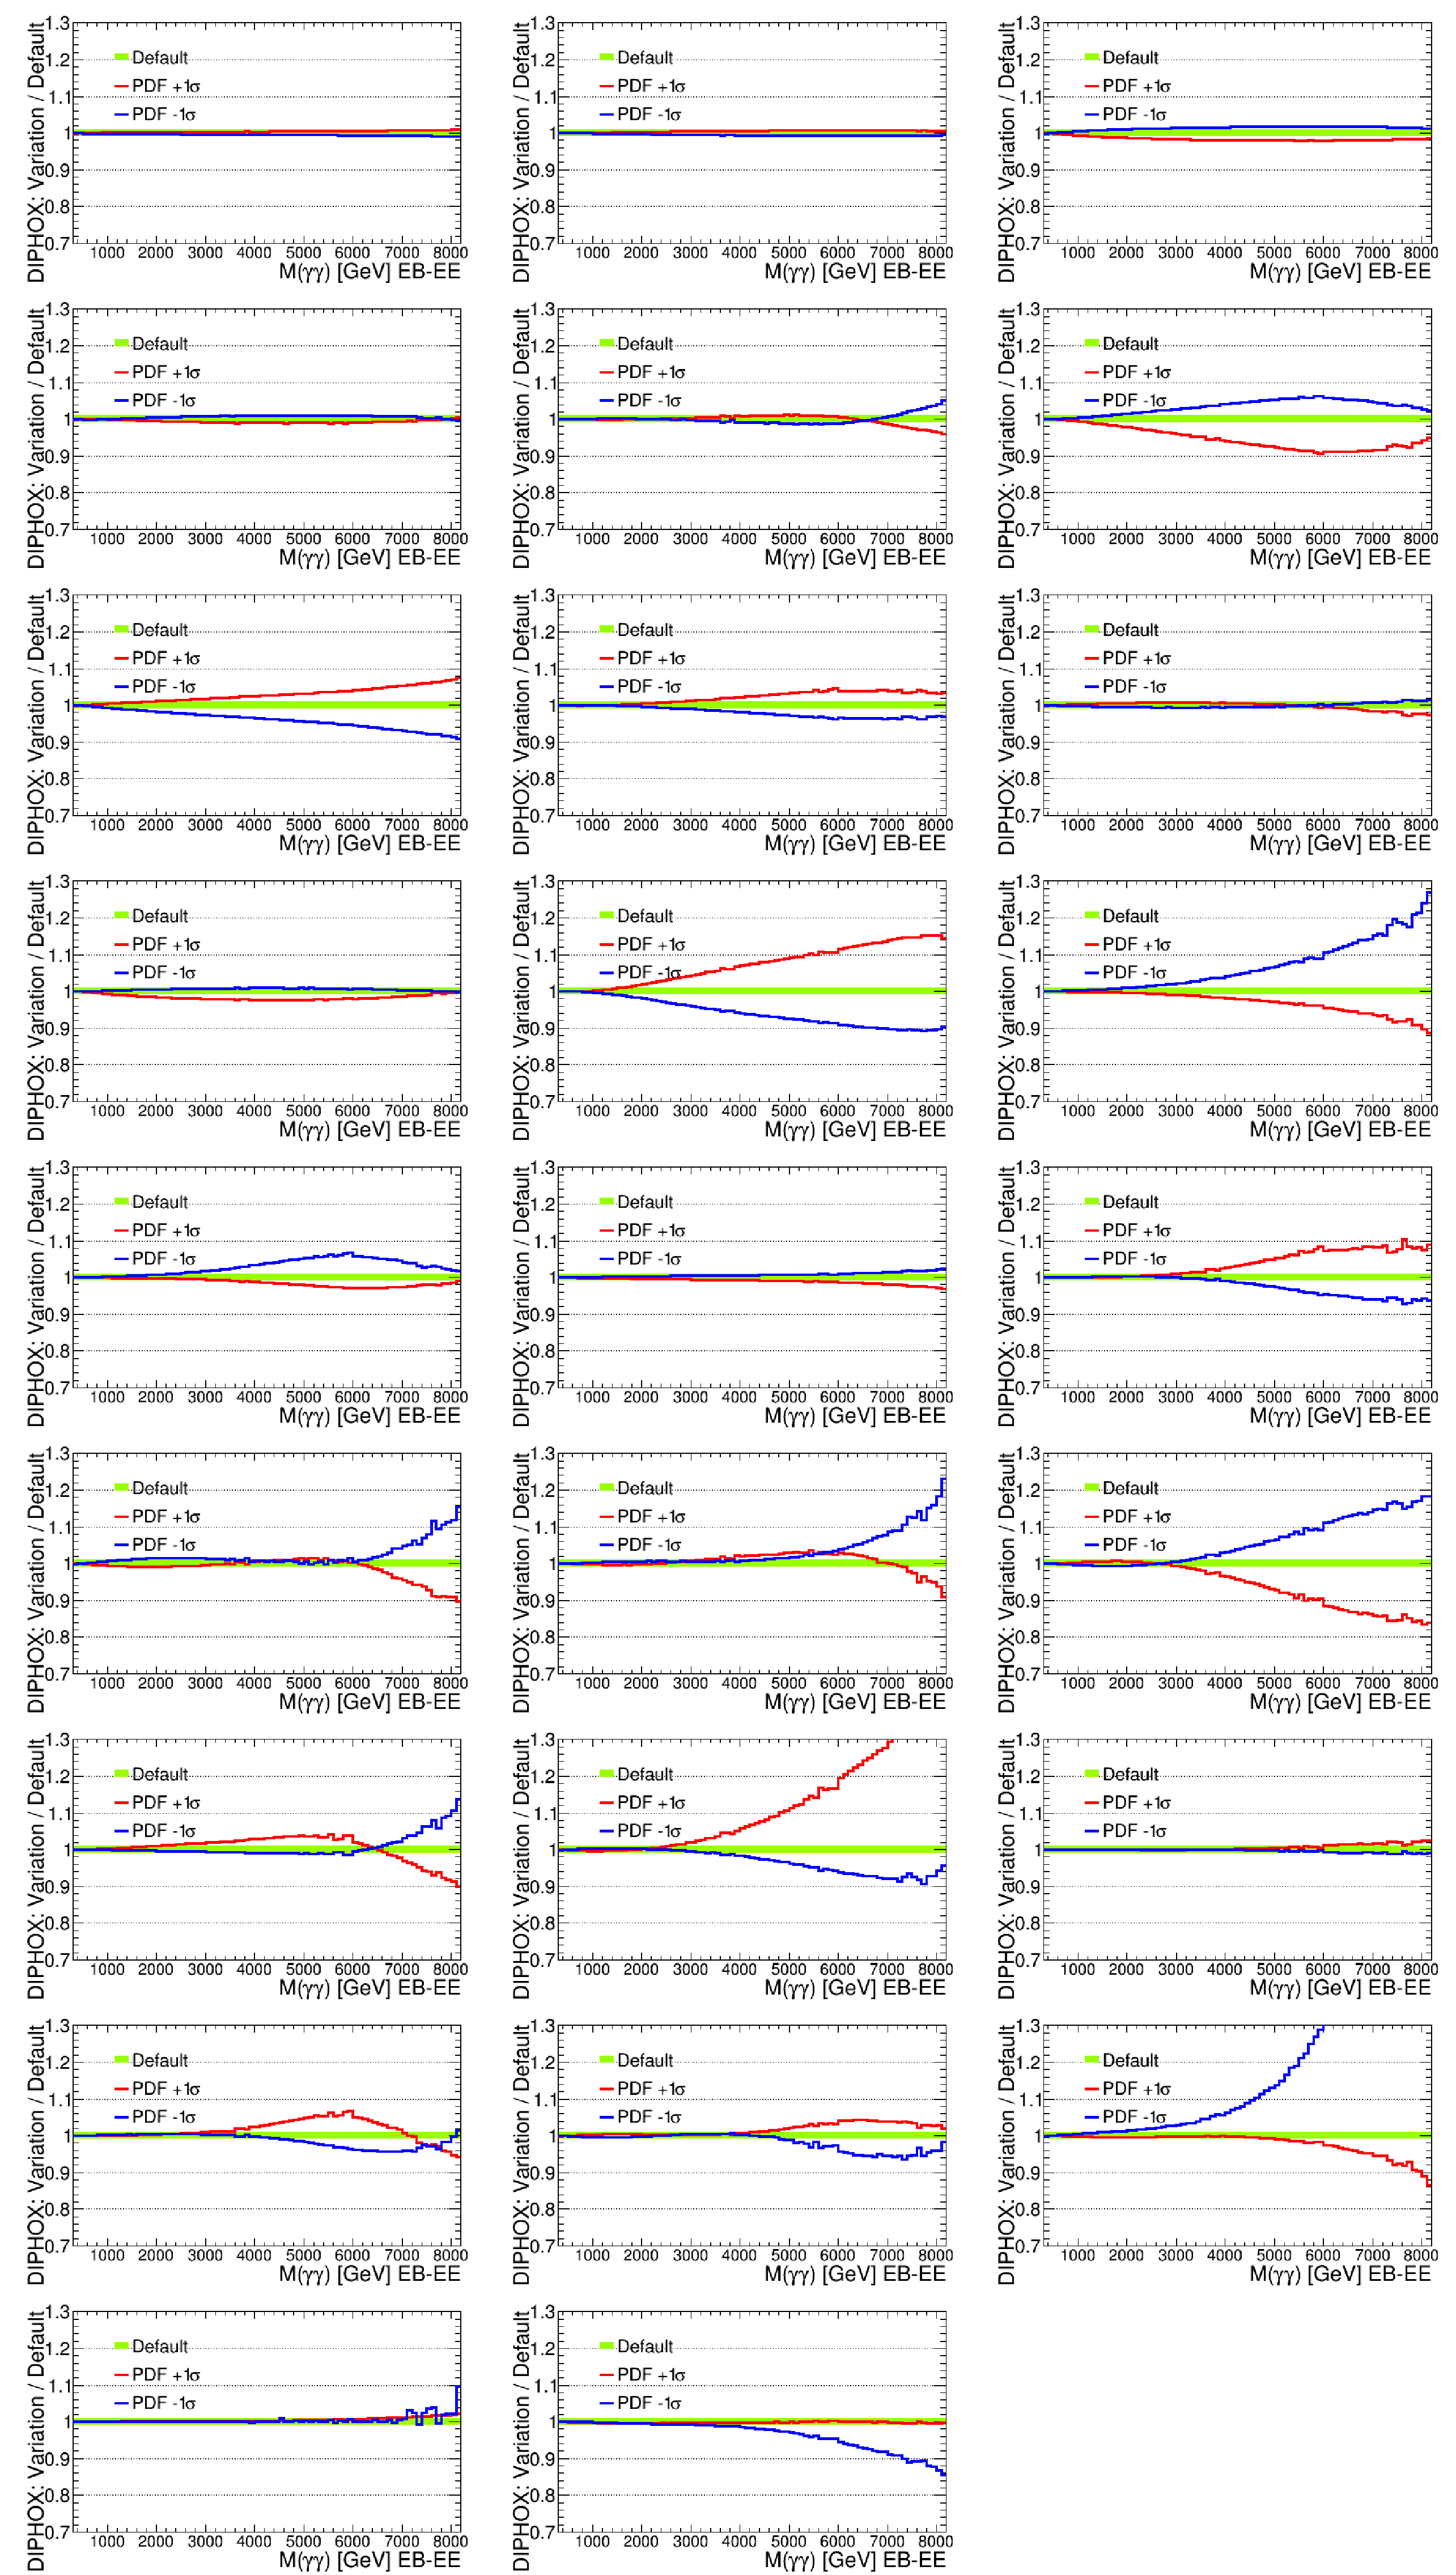
\includegraphics[scale=0.27]{figures/SYS_PDF_EE.pdf}
	\caption{The $\pm1$ standard deviation variations of each of the 26 PDF eigenvectors in the EBEE category. Each distribution is the ratio of the variation over the default prediction as a function of \mgg.}
	\label{fig:sys_PDF_EE}
\end{figure}

Another source of systematic uncertainty considered on the background shape is the difference in shape between the NNLO \MCFM \mgg spectra and of the shapes predicted at NLO by \MCFM and \DIPHOX. This is determined by comparing the shapes of the \MCFM NNLO and the \MCFM NLO predictions (used as the positive variation) and between the \MCFM NNLO and \DIPHOX NLO predictions (used as the negative variation). This is done to provide a conservative bound on the effects of the absent higher order terms.

Uncertainties due to the photon energy scale and resolution have a negligible impact on this nonresonant search.


\section{Fake Background Systematic Uncertainties}

A systematic uncertainty of 30\% is assigned to the normalization of the fake background measurement from the variation of the fake rake as a function of pileup, photon $\eta$, a change of the sideband definition, and a change of template variable. In addition, this covers the degree of variation observed in the fake rate method from the closure test, including any potential real photon contamination. A separate systematic uncertainty on the shape of the fake background is applied to account for the difference in shape between the fake rate measurements constructed using the jet- and muon-triggered datasets. This shape uncertainty makes a subdominant contribution. The details of these studies were presented in Section~\ref{sec:fake_background}.


\section{Signal Systematic Uncertainties}

Systematic uncertainties are assigned to the normalization of the signal calculation to account for the uncertainties in measurements of the integrated luminosity and overall diphoton selection efficiency, corresponding to 2.5\%~\cite{CMS-PAS-LUM-17-001} and 6\%, respectively. The selection efficiency includes the trigger and high-\pt photon ID efficiency, which are 3\% per photon. The PDF uncertainties affecting the signal shape are determined using the same procedure as is done for the background, by separately varying the 26 eigenvalue pairs using \DIPHOX at NLO. These PDF uncertainties are assumed to be 100\% correlated between the signal and background. The effect of the PDF uncertainty on the signal cross section is considered a theoretical uncertainty and not treated as a systematic uncertainty.


\section{Summary of the Systematic Uncertainties}

A summary of the dominant systematic uncertainties as a function of \mgg in the EBEB and EBEE categories is shown in Fig.~\ref{fig:sys_unc}. Here, the uncertainties are added in quadrature and shown as fraction of the total yields. The colored bands represent the dominant pre-fit systematic uncertainties, i.e., before the fit of the background normalization, constrained by the data. The pre-fit systematic uncertainties do not included the normalization of the SM diphoton prediction or the NLO shapes, and, therefore, the black and red curves cannot be directly compared. At high-\mgg, the PDF uncertainties are dominant. The total post-fit systematic uncertainty is also shown in each category. At high-\mgg, these are driven upward primarily due to their influence under the shape and normalization of the data. A decomposition of the total post-fit uncertainty into its individual components is limited by the choice of fitting framework used. However, the the variation of each post-fit systematic uncertainty will be described and shown in Chapter~\ref{ch:results}, during the discussion of the fitting procedure.

\begin{figure}[!htbp]
	\centering
	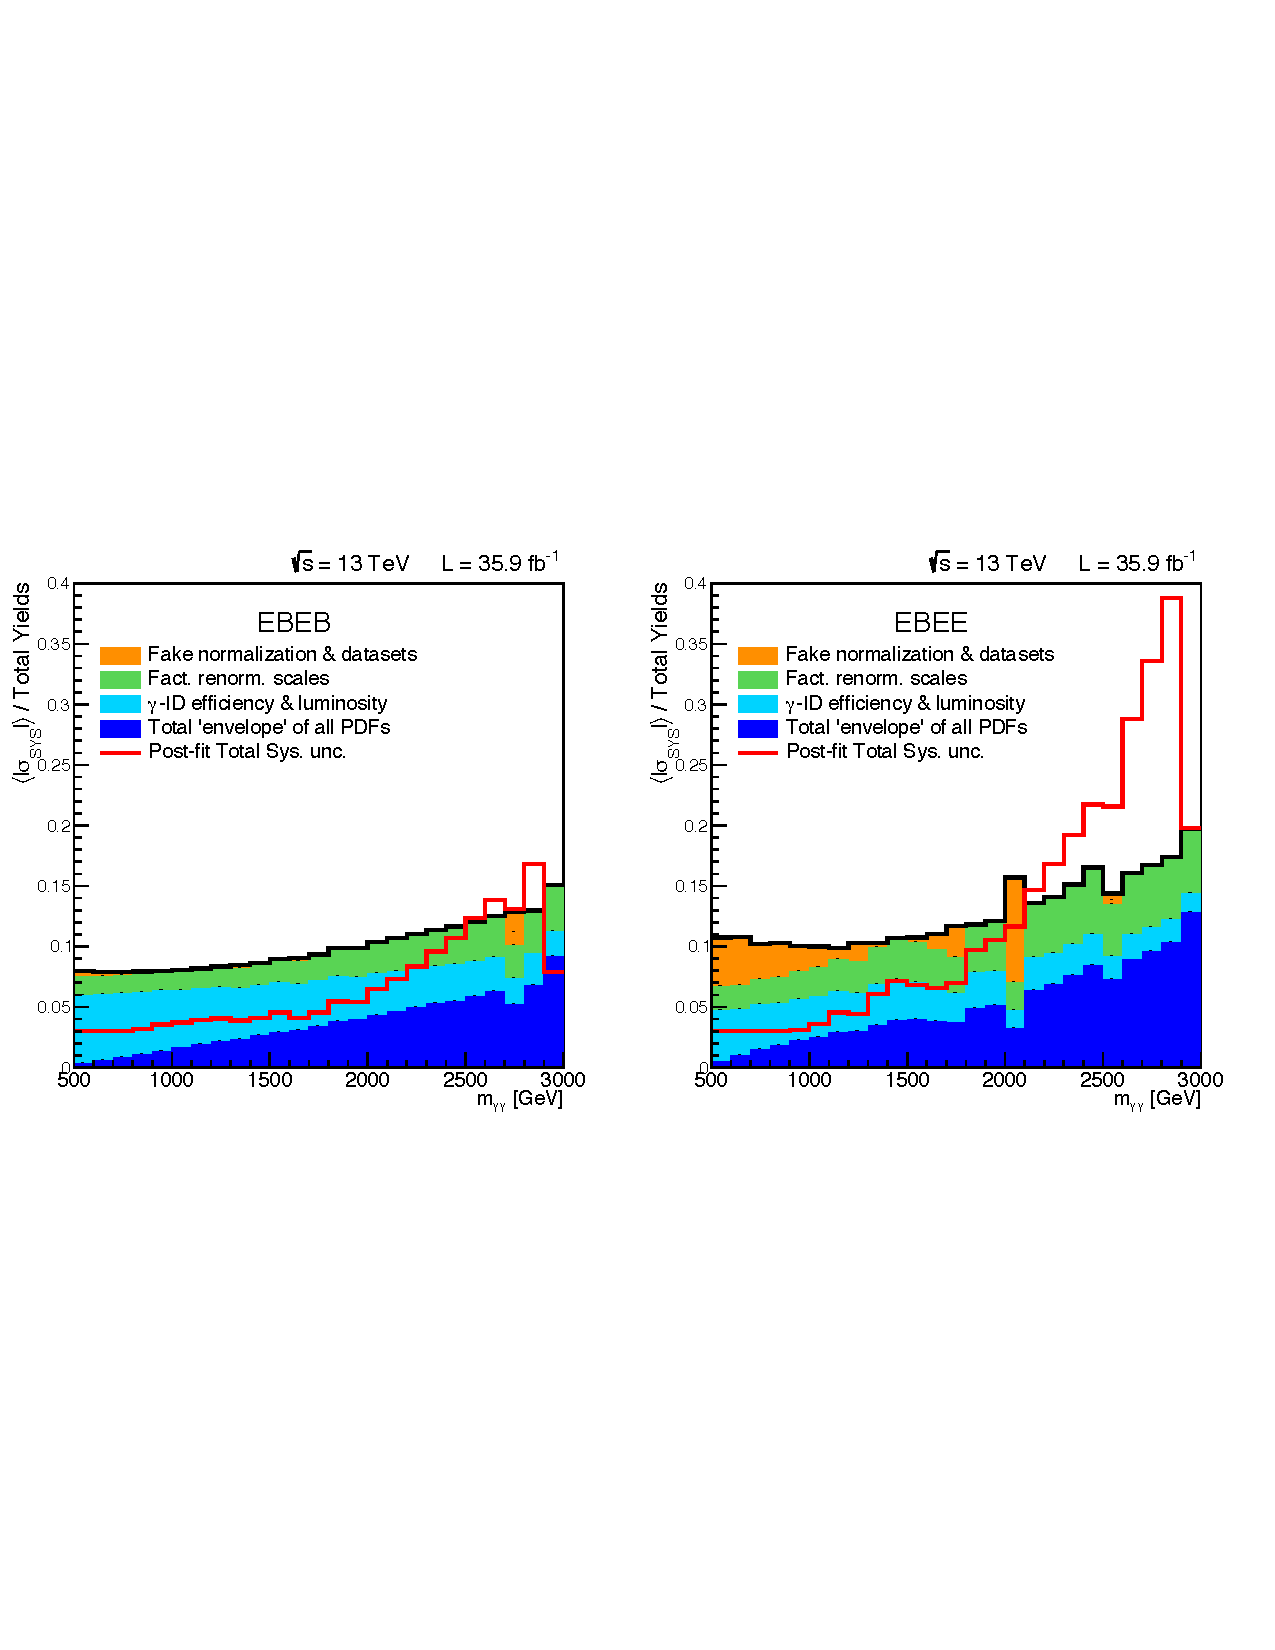
\includegraphics[width=1.0\textwidth]{figures/PLOT_PRED_PULL_SYS.pdf}
	\caption{The dominant pre-fit systematic uncertainties and total post-fit uncertainty as a function of \mgg in the EBEB (left) and EBEE (right) categories.}
	\label{fig:sys_unc}
\end{figure}




